%\documentclass[tikz, border=5pt]{standalone}
\begin{document}
	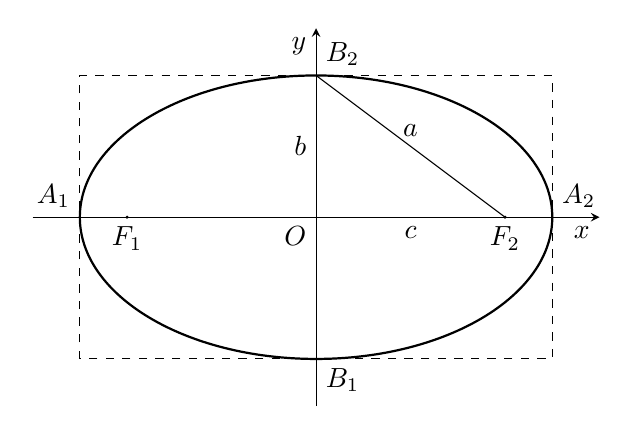
\begin{tikzpicture}[>=stealth, scale=0.6]
		% 1. 定义椭圆参数(长半轴a=5,短半轴b=3,焦距c=4,满足c=√(a²-b²))
		\def\a{5}  % 长半轴
		\def\b{3}  % 短半轴
		\def\c{4} % 焦距(近似√(5²-3²)=√16≈4)
		
		% 2. 绘制辅助矩形(虚线)
		\draw[dashed] (-\a, -\b) rectangle (\a, \b);
		
		% 3. 绘制椭圆
		\draw[thick] (0,0) ellipse ({\a} and {\b});
		
		% 4. 绘制坐标轴
		\draw[->] (-\a-1,0) -- (\a+1,0) node[below left] {$x$};
		\draw[->] (0,-\b-1) -- (0,\b+1) node[below left] {$y$};
		\node at (0,0) [below left] {$O$}; % 原点
		
		% 5. 标记顶点与焦点
		\node at (-\a,0) [above left] {$A_1$};   % 左顶点
		\node at (\a,0)  [above right] {$A_2$};  % 右顶点
		\node at (0,\b)  [above right] {$B_2$};  % 上顶点
		\node at (0,-\b) [below right] {$B_1$};  % 下顶点
		\fill (-\c,0) circle (1pt) node[below] {$F_1$}; % 左焦点
		\fill (\c,0) circle (1pt) node[below] {$F_2$}; % 右焦点
		
		% 6. 绘制线段 B2F2
		\draw (0,\b) -- (\c,0);
		
		% 7. 标记线段长度(a, b, c)
		\node at (2,1.5) [above] {$a$};  % 线段 B2F2 标注为 a
		\node at (0,1.5) [left] {$b$};  % 从 O 到 B2 标注为 b
		\node at (2,0) [below] {$c$}; % 从 O 到 F2 标注为 c
	\end{tikzpicture}
\end{document}
